\documentclass[xcolor={table}]{beamer}
%\usetheme{Lapesd}
\usepackage{./sty/beamerthemeLapesd}

\usepackage{morewrites}

\usepackage[brazilian]{babel}	% coloca as coisas em portugues no sumário.
\usepackage[utf8]{inputenc}
\usepackage[T1]{fontenc}
\usepackage[scaled]{helvet}
\usepackage{amsthm}
\usepackage{ragged2e}
% \usepackage{subfig}
\usepackage[table]{xcolor}
\usepackage{ctable}
\usepackage{multicol}
\usepackage{multirow}
\usepackage{fancyvrb}
\usepackage{subcaption}
\usepackage{listings}
\usepackage{color}
\usepackage[font={scriptsize,it}]{caption}
\renewcommand{\lstlistingname}{Code}
\definecolor{lightgray}{rgb}{0.97,0.97,0.97}
\definecolor{lightred}{rgb}{1,0.7,0.7}

\lstdefinelanguage{cc}{
    language     = C++,
    morekeywords = {Array2D, __parallel__, Mask2D, Stencil2D}
}

\lstdefinestyle{highlight}{
    numbers=none,
    stepnumber=1,
    numbersep=-8pt,
    numberstyle=\small\color{black},
    basicstyle=\scriptsize\ttfamily\color{black},
    keywordstyle=\color{blue},
    commentstyle=\color{black},
    stringstyle=\color{black},
    numberstyle=\footnotesize\ttfamily\color{black},
    escapeinside={(*}{*)},
    tabsize=2,
    language=cc, %morecomment=[l][{\color[rgb]{0.1, 0.2, 0.8}}]{},
    %aboveskip=0.1in, % space before the caption
    %belowskip=0.1in, % space after listing
    captionpos=b,
    showstringspaces=false,
    %belowcaptionskip=1\baselineskip,
    %breaklines=true,
    %moredelim=[l][\color{blue}]{\#pragma},
    % backgroundcolor=\color{white}
}

\lstdefinestyle{base}{
    numbers=none,
    stepnumber=1,
    numbersep=-8pt,
    morekeywords={Array2D, \_\_parallel\_\_, Mask2D, Stencil2D}
    numberstyle=\small\color{black!40},
    basicstyle=\scriptsize\ttfamily\color{black!40},
    keywordstyle=\color{blue!40},
    commentstyle=\color{black!40},
    stringstyle=\color{black!40},
    numberstyle=\footnotesize\ttfamily\color{black!40},
    escapeinside={(*}{*)},
%     frame=none, %single
    tabsize=2,
    language=cc, %morecomment=[l][{\color[rgb]{0.1, 0.2, 0.8}}]{},
    %aboveskip=0.1in, % space before the caption
    %belowskip=0.1in, % space after listing
    captionpos=b,
    showstringspaces=false,
    %belowcaptionskip=1\baselineskip,
    %breaklines=true,
    %moredelim=[l][\color{blue}]{\#pragma},
    % backgroundcolor=\color{white!40}
    moredelim=**[is][\only<+>{\color{black}\lstset{style=highlight}}]{@}{@},
}

% \lstdefinestyle{highlight}{
    % keywordstyle=\color{red},
    % commentstyle=\color{green},
% }
% \lstdefinestyle{base}{
    % language={C++},
    % basicstyle=\color{black!40},
    % keywordstyle=\color{red!40},
    % commentstyle=\color{green!40},
    % moredelim=**[is][\only<+>{\color{black}\lstset{style=highlight}}]{@}{@},
% }

\newcommand{\Fw}{\textit{Framework}\xspace}
\newcommand{\fw}{\textit{framework}\xspace}
\newcommand{\Fws}{\textit{Frameworks}\xspace}
\newcommand{\fws}{\textit{frameworks}\xspace}

\newcommand{\pskel}{PSkel\xspace}
\newcommand{\mppa}{MPPA-256\xspace}

\graphicspath{{./figs/}}
\DeclareGraphicsExtensions{.pdf,.jpg,.png,.gif}

\def\signed #1{{\leavevmode\unskip\nobreak\hfil\penalty50\hskip2em
        \hbox{}\nobreak\hfil(#1)
        \parfillskip=0pt \finalhyphendemerits=0 \endgraf}}

\renewcommand{\footnotesize}{\tiny}

\newcommand{\mymacro}[1]{#1}

\addtobeamertemplate{block begin}{}{\justifying}

\captionsetup{labelformat=simple}
\captionsetup[table]{belowskip=0pt}

\title[Comparação de Tecnologias de Comunicação no MPPA-256]{
   \textbf{Comparação de Tecnologias de Comunicação entre Clusters no Processador MPPA-256: Um Estudo com Aplicações do CAP Benchmarks}}
\author[Grunheidt, D.]{\textbf{David Grunheidt Vilela Ordine}, Márcio Castro}
\date{27 de dezembro de 2020}
\institute{Departamento de Informática e Estatística (INE)\\ Universidade Federal de Santa Catarina (UFSC)\\ 
\url{david.ordine@grad.ufsc.br} \\ \url{marcio.castro@ufsc.br}}

\begin{document}
\begingroup
    \makeatletter
    \setlength{\hoffset}{-0.5\beamer@sidebarwidth}
    \makeatother
    \begin{frame}[plain,t,noframenumbering]
        \titlepage
    \end{frame}
\endgroup

%=============================================================================================

\section{Sumário}
\begin{frame}\frametitle{Sumário}
    \begin{itemize}
        \item Introdução
        \item Fundamentação Teórica
        \item Desenvolvimento
        \item Resultados
        \item Conclusão
    \end{itemize}
    \vfill
\end{frame}

\section{Introdução}
\begin{frame}\frametitle{Contexto}
    \begin{itemize}
        \item{Objetivo de alcançar a computação em \textit{Exascale}}
        \item{Viável - 50 GFlops/W X Máximo - 14.719 GFlops/W}
        \item{\textit{Trade-off} desproporcional entre desempenho e consumo energético (barreira de potência)}
        \begin{figure}[tb]
            \centering
            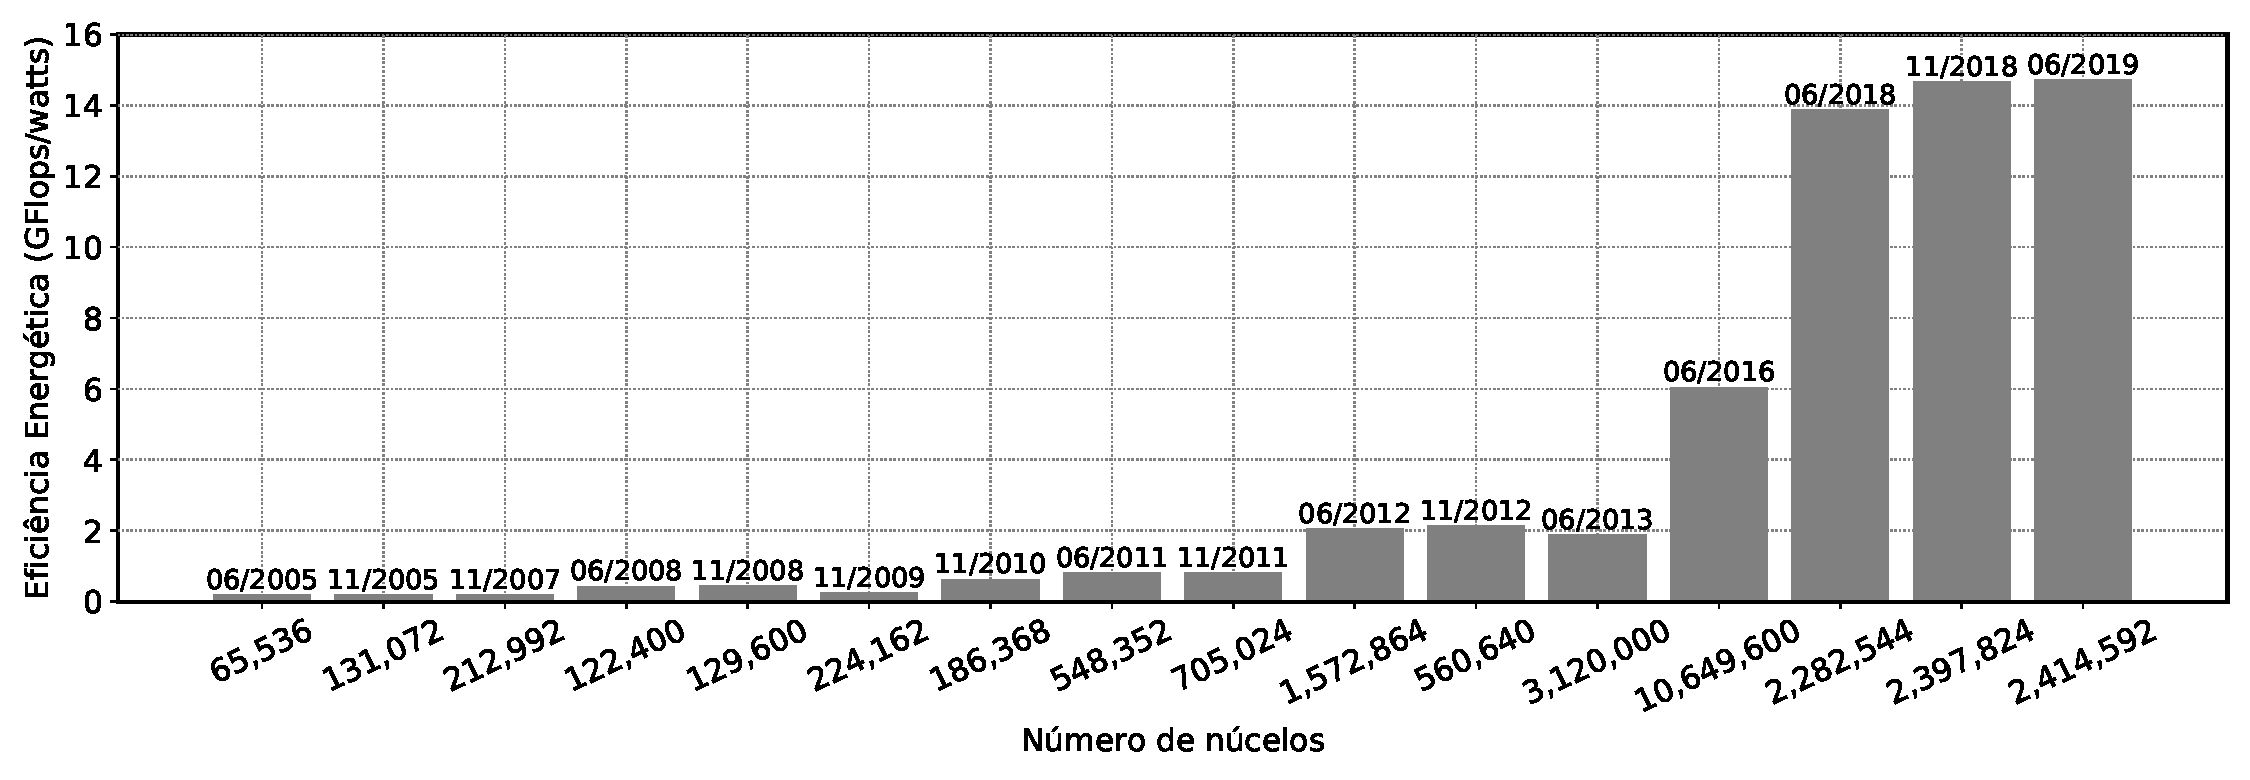
\includegraphics[width=1\linewidth, keepaspectratio]{figs/Figure_Efficiency_X_Cores_Top500.pdf}
            \caption{Eficiência energética X número de núcleos do TOP1 supercomputador do \textit{ranking} TOP500 ao passar dos anos.}
            \label{fig:eficienciaxcorestop500}
        \end{figure}
    \end{itemize}
    \vfill
\end{frame}

\begin{frame}\frametitle{Contexto}
    \begin{itemize}
        \item{Processadores \textit{manycore} de baixa potência como solução do problema}
        \begin{itemize}
            \item {MPPA-256 \cite{MPPA-2:2013}}
            \item {Adapteva Epiphany \cite{Olofsson2014}}
            \item {SW26010 (\textit{Sunway TaihuLight}) \cite{sunway:2016}}
        \end{itemize}
        \item MPPA-256 como objeto de estudo deste trabalho
        \item {Necessário avaliar seu desempenho:}
        \begin{itemize}
            \item CAP-Benchmarks
        \end{itemize}
    \end{itemize}

    \vfill
\end{frame}

\begin{frame}\frametitle{Contexto}
    \begin{itemize}
        \item {Duas versões do \textit{benchmark}:}
        \begin{itemize}
            \item \textit{MPPA Interprocess Communication API} (IPC)
            \item \textit{MPPA Asynchronous Communication API} (ASYNC)
        \end{itemize}
        \item {\textbf{Objetivos:}}
        \begin{itemize}
            \item Portar aplicações do CAP-Bench para a API ASYNC
            \item Avaliar os custos e benefícios do MPPA-256 (tempos de execução, gasto energético e tráfego de dados)
            \item Comparar as tecnologias IPC e ASYNC
            \item Estudar as peculiaridades de cada tecnologia
        \end{itemize}
    \end{itemize}
    \vfill
\end{frame}

\section{Fundamentação Teórica}
\subsection{MPPA-256}
\begin{frame}\frametitle{MPPA-256}
    \begin{itemize}
        \item{16 \textit{clusters} de computação (CCs)}
        \begin{itemize}
            \item 16 núcleos em cada CC, atuando a 400 Mhz cada
            \item Memória compartilhada de 2MB
            \item Memória cache associativa 2-way, privadas e de 32 kB
        \end{itemize}
        \item{4 \textit{clusters} de E/S}
        \begin{itemize}
            \item 4 núcleos gerenciadores de recursos em cada
        \end{itemize}
        \begin{figure}
            \centering
            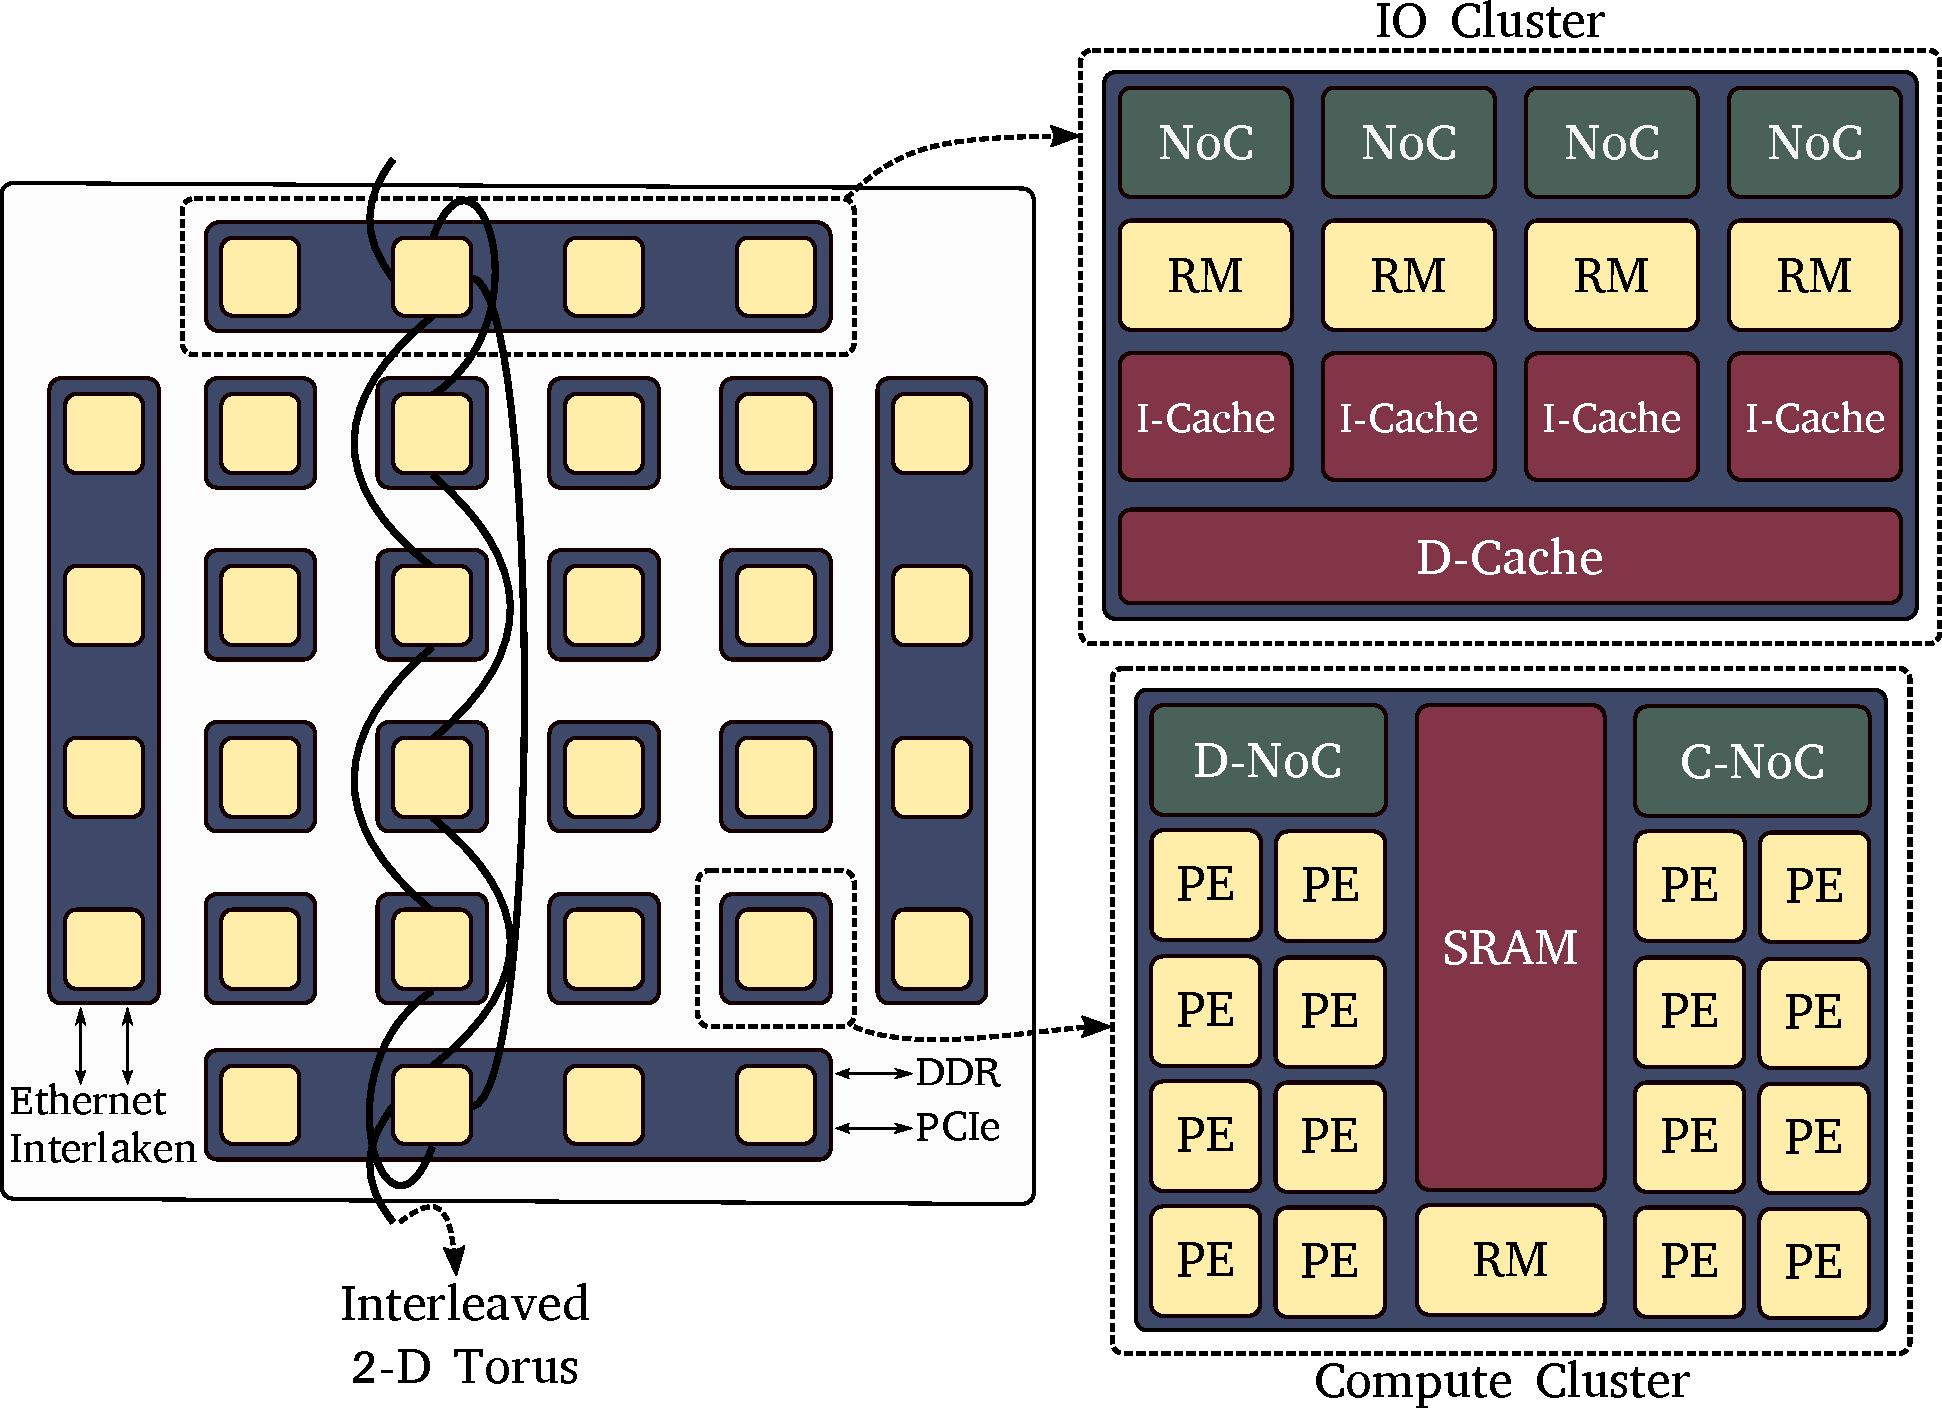
\includegraphics[width=5cm, keepaspectratio]{figs/mppa-overview.pdf}
            \caption{Visão arquitetural do MPPA-256 \cite{Penna2018}}
            \label{fig:arquiteturamppa}
        \end{figure}
    \end{itemize}
\end{frame}

\subsection{OpenMP API}
\begin{frame}\frametitle{Open Multi-Processing}
    \begin{itemize}
        \item Implementação de aplicações paralelas
        \begin{itemize}
            \item C, C++ e Fortran
        \end{itemize}
        \item Voltada ao \textit{multithreading}
        \item Centrada no modelo Fork-Join
        \begin{figure}[tb]
          \centering
          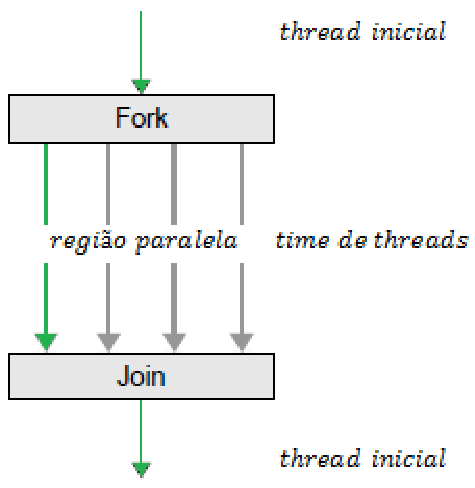
\includegraphics[width=.4\linewidth, keepaspectratio]{figs/forkjoin.pdf}
          \caption{Esquema do modelo \textit{fork-join}.}
          \label{fig:forkjoin}
        \end{figure}
    \end{itemize}
\end{frame}

\begin{frame}\frametitle{Open Multi-Processing}
    \begin{itemize}
        \item Diretivas de compilação e regiões paralelas
        \begin{itemize}
            \item \#pragma omp parallel for
        \end{itemize}
        \begin{figure}[tb]
          \centering
          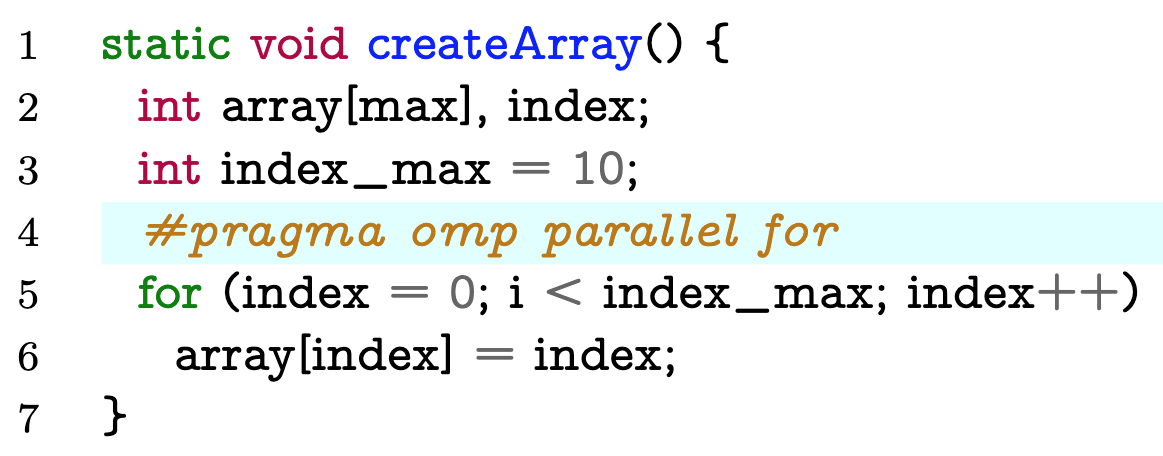
\includegraphics[width=.8\linewidth, keepaspectratio]{figs/loopopenmp.png}
          \caption{Execução de um \textit{loop} de forma paralela.}
          \label{lst:parallelloop}
        \end{figure}
    \end{itemize}
\end{frame}

\begin{frame}\frametitle{Open Multi-Processing}
    \begin{itemize}
        \item Cláusulas OpenMP
        \begin{itemize}
            \item private, default e reduction
        \end{itemize}
        \begin{figure}[tb]
          \centering
          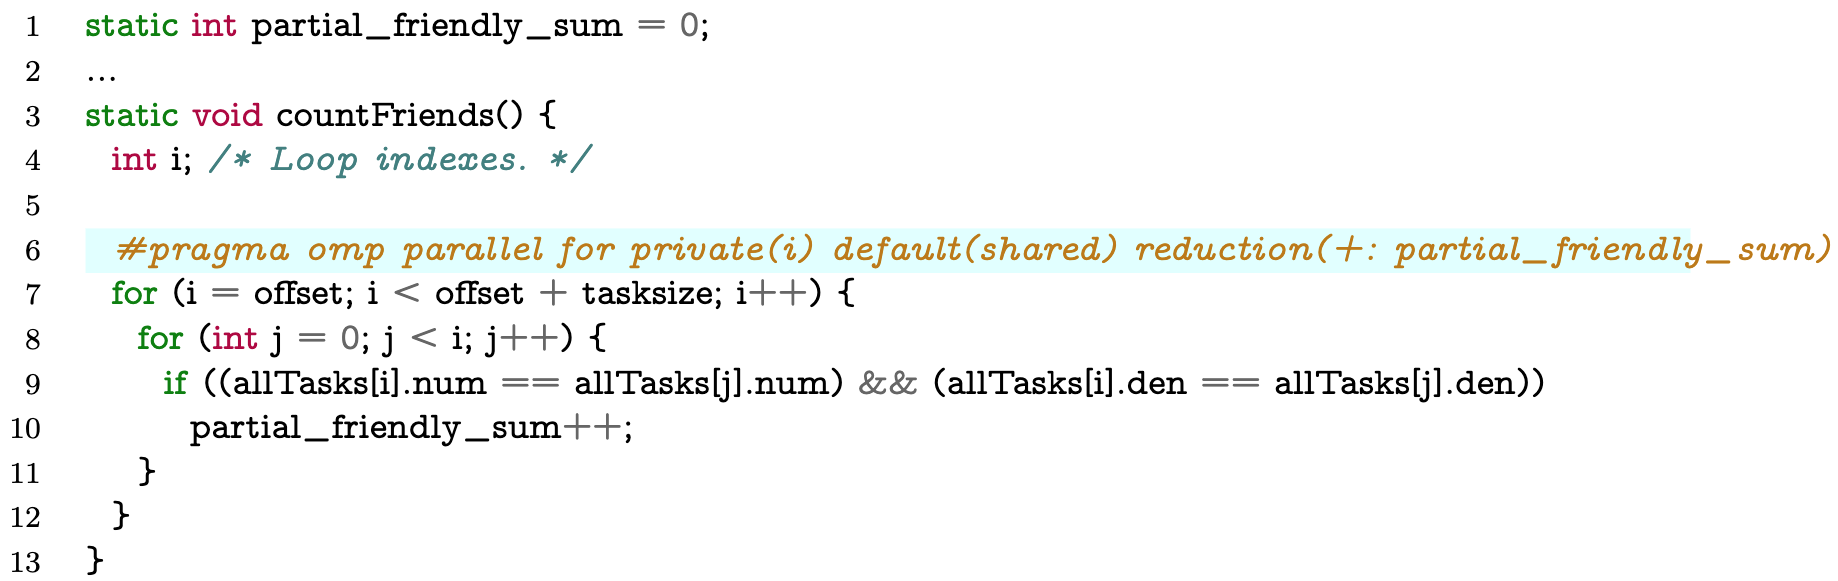
\includegraphics[width=1\linewidth, keepaspectratio]{figs/reductionloop.png}
          \caption{Exemplo de leitura e armazenamento seguro em variável compartilhada entre \textit{threads} em uma das aplicações do CAP-Bench.}
          \label{lst:reductionloop}
        \end{figure}
    \end{itemize}
\end{frame}

\subsection{Modelo mestre-escravo}
\begin{frame}\frametitle{Modelo mestre-escravo no MPPA-256}
    \begin{itemize}
        \item \textit{Clusters} de E/S gerenciam os \textit{clusters} de computação
        \item Execução de códigos binários diferentes
        \item Cada cluster executa um código paralelizado com OpenMP 
        \begin{figure}[tb]
          \centering
          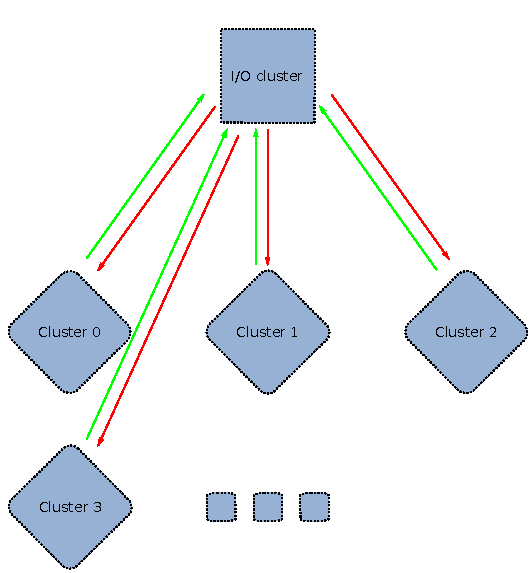
\includegraphics[width=.4\linewidth, keepaspectratio]{figs/mppamasterslave.pdf}
          \caption{Fluxo de uma aplicação seguindo o modelo \textit{mestre-escravo} no MPPA-256.}
          \label{fig:masterslave}
        \end{figure}
    \end{itemize}
\end{frame}

\subsection{MPPA IPC API}
\begin{frame}\frametitle{MPPA IPC API}
    \begin{itemize}
        \item Definir caminhos de comunicação explicitamente
        \item Controle dos caminhos é feito pelo programador
        \item Conhecimento profundo da arquitetura
        \begin{figure}[tb]
          \centering
          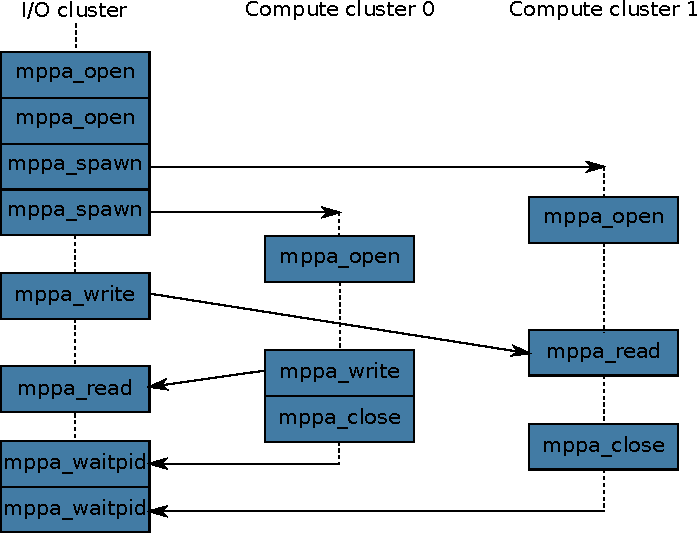
\includegraphics[width=.6\linewidth, keepaspectratio]{figs/mppaipcflow.pdf}
          \caption{Fluxo de uma aplicação usando funções do tipo POSIX da IPC no MPPA-256.}
          \label{fig:mppaipcflow}
        \end{figure}
    \end{itemize}
\end{frame}

\subsection{MPPA ASYNC API}
\begin{frame}\frametitle{MPPA ASYNC API \cite{Hascoet2017}}
    \begin{itemize}
        \item {Comunicação assíncrona e unilateral entre \textit{clusters}}
        \item {Segmentos sobre espaços locais de memória}
        \begin{itemize}
            \item Abstração do modelo de memoria distribuída
            \item Clonagem de segmentos
            \item Operações \textit{put/get} sobre segmentos
        \end{itemize}
        \begin{figure}
            \centering
            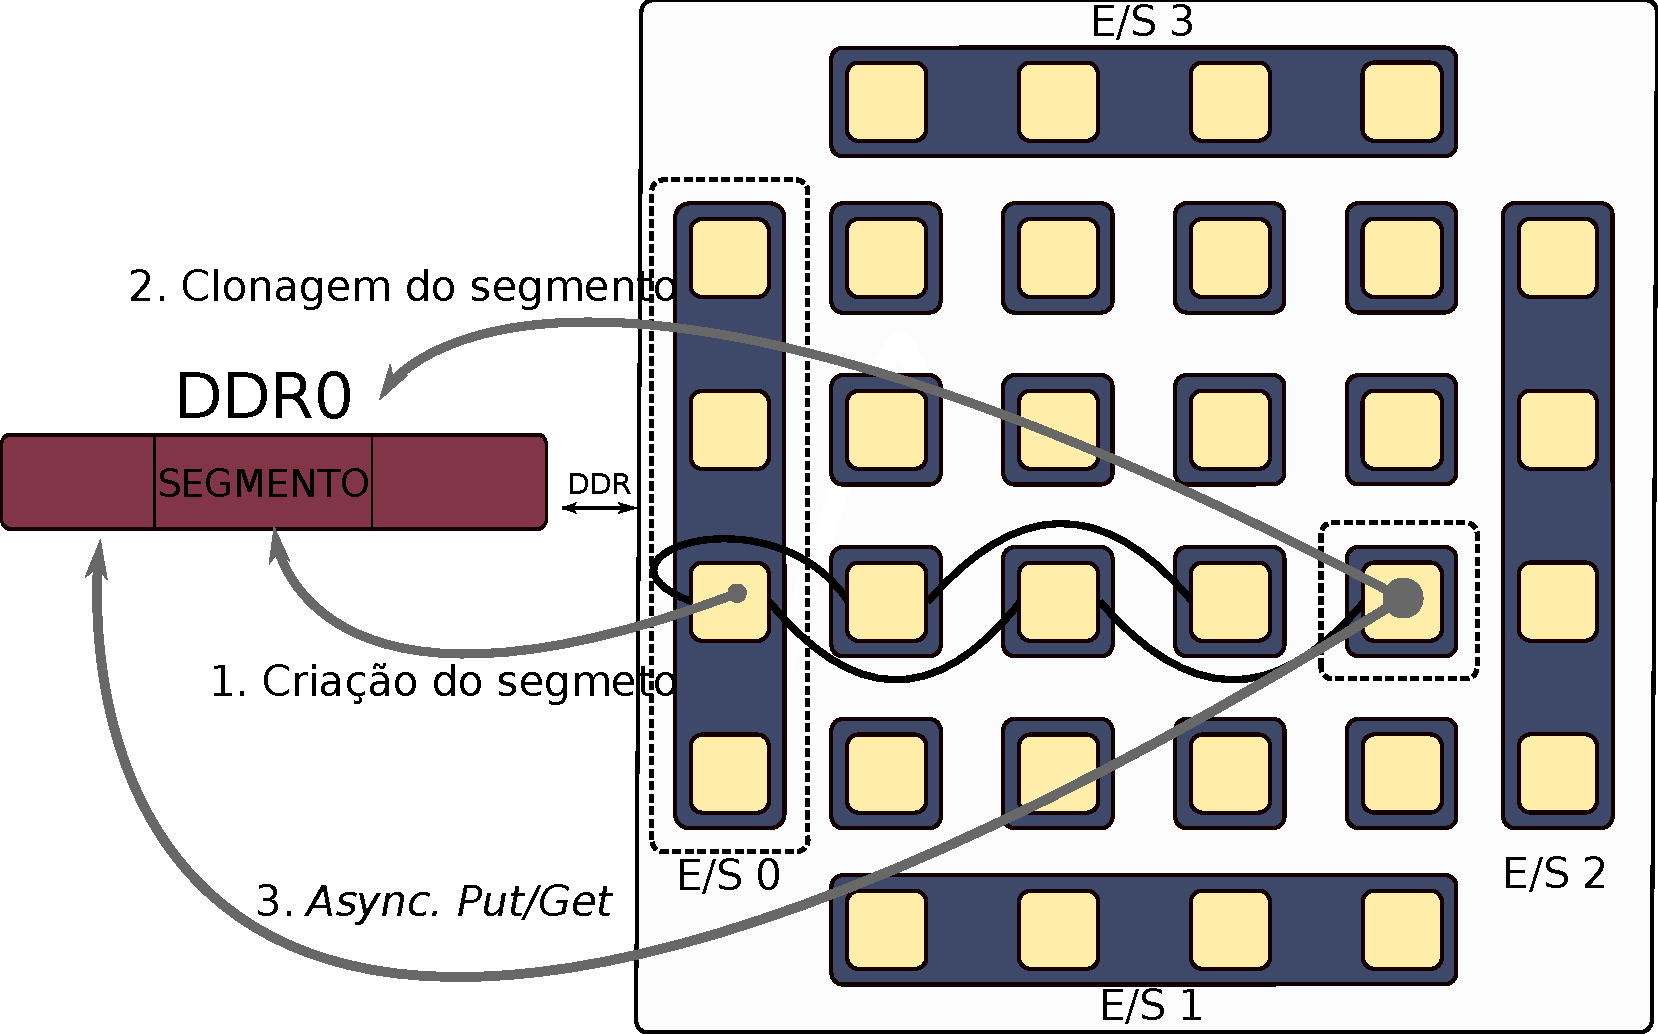
\includegraphics[width=.6\linewidth, keepaspectratio]{figs/putget.pdf}
            \caption{Visão esquemática do funcionamento da biblioteca \textit{async}}
            \label{fig:putget}
        \end{figure}
    \end{itemize}
\end{frame}

\subsection{CAP-Benchmarks}
\begin{frame}\frametitle{CAP-Benchmarks \cite{Castro-Souza-CCPE:2016}}
    \begin{itemize}
        \item {Conjunto de 7 aplicações desenvolvidas em C}
        \begin{itemize}
            \item {Uma das aplicações não foi portada neste trabalho}
        \end{itemize}
    	\item {Domínios de problemas variados}
    	\item {Diferentes padrões paralelos}
    	\item {Testar o processador em diversas condições}
        \item {Criado para avaliar diferentes processadores de arquitetura \textit{Manycore}}
    \end{itemize}
\end{frame}

\section{Desenvolvimento}
\begin{frame}\frametitle{Desenvolvimento}
    \begin{itemize}
        \item Fluxo de desenvolvimento de cada aplicação
        \begin{itemize}
            \item Alterações de otimização
            \item Alterações de tecnologia de comunicação
        \end{itemize}
        \item Otimizações valem para ambas as versões
        \item Comparação dos resultados leva em conta somente a tecnologia
    \end{itemize}
\end{frame}

\subsection{Friendly Numbers}
\begin{frame}\frametitle{Friendly Numbers}
    \begin{itemize}
        \item Dois números naturais são amigáveis se compartilham a mesma abundância
        \item {Abundância $\mathnormal{A}$ de um número $\mathnormal{n}$ -> $\mathnormal{A(n) = \frac{\sigma(b)}{n}}$}
        \begin{itemize}
            \item {$\sigma(n)$ representa a soma de todos os divisores de n}
        \end{itemize}
        \item Calcula e compara as abundâncias de números em um intervalo
        \item Quais pares de números são amigáveis neste intervalo?
    \end{itemize}
\end{frame}

\begin{frame}\frametitle{Alterações no FN}
    \begin{itemize}
        \item {Segmento sobre o \textit{array} de tarefas}
        \item {Operações de PUT/GET somente nos \textit{slaves}}
        \item {Otimização na função de soma dos divisores}
        \begin{itemize}
            \item {Antes: loop entre 2 e o número}
            \item {Agora: loop entre 2 e metade do número}
        \end{itemize}
        \item {POSIX \textit{Threads} -> OpenMP}
        \begin{itemize}
            \item Implementação do paralelismo reduzido: 50 linhas -> 5.
        \end{itemize}
        \begin{figure}
            \centering
            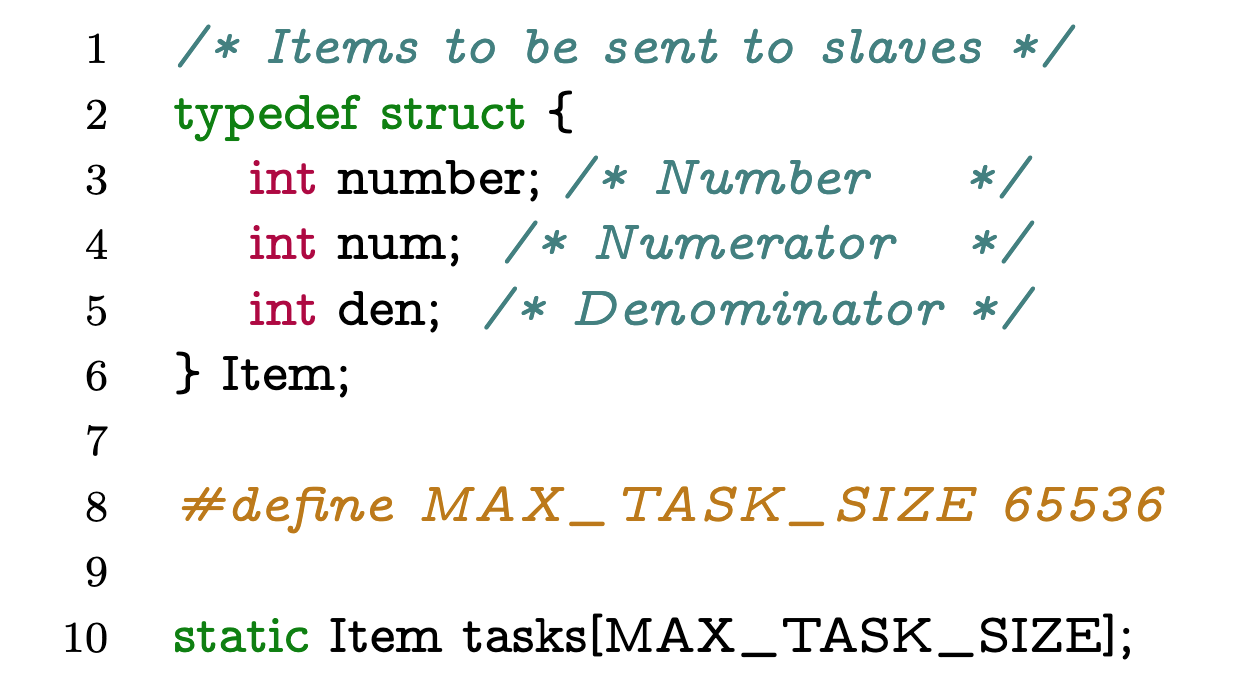
\includegraphics[width=.5\linewidth, keepaspectratio]{figs/fnstructitemtask.png}
            \caption{Definição das tarefas por  parte do \textit{cluster} de IO.}
            \label{lst:structitemtask}
        \end{figure}
    \end{itemize}
\end{frame}

\subsection{Fast}
\begin{frame}\frametitle{Features from Accelerated Segment Test}
    \begin{itemize}
        \item {Algoritmo de detecção de cantos}
        \item {Extrair pontos importantes em uma imagem}
        \item {Círculo de 16 \textit{pixels} testa se um ponto $\mathnormal{p}$ é um canto}
        \item {Brilho de um \textit{pixel} é um inteiro entre 1 e 16}
        \item {É canto se:}
        \begin{itemize}
            \item {Brilho dos $\mathnormal{N}$ \textit{pixels} do círculo > brilho de $\mathnormal{p}$ + limiar $\mathnormal{t}$}
            \item {Brilho dos $\mathnormal{N}$ \textit{pixels} do círculo < brilho de $\mathnormal{p}$ - limiar $\mathnormal{t}$}
        \end{itemize}
    \end{itemize}
\end{frame}

\begin{frame}\frametitle{Alterações no FAST}
    \begin{itemize}
        \item {Versão antiga}
        \begin{itemize}
            \item {Tarefas enviadas explicitamente aos CCs}
            \item {CCs aguardavam em um \texttt{while(true)}}
            \item {Mensagens sinalizando continuação ou finalização}
        \end{itemize}
        \item {Nova versão}
        \begin{itemize}
            \item {CCs sabem exatamente a quantidade de tarefas a serem realizadas}
            \item {Solicitam tarefas ao \textit{cluster} de I/O}
            \item {Mensagens do \textit{master} para um \textit{slave}: Redução 4 -> 1}
            \item {Mensagens de um \textit{slave} para o \textit{master}: Redução 2 -> 1}
        \end{itemize}
        \item {Inversão da lógica de tarefas garante grande paralelismo}
    \end{itemize}
\end{frame}

\subsection{Gaussian Filter}
\begin{frame}\frametitle{Gaussian Filter}
    \begin{itemize}
        \item {Algoritmo que aplica um filtro de suavização em uma imagem}
        \item {Poucas alterações entre versões do CAP-Bench}
        \item {Dois segmentos criados}
        \begin{itemize}
            \item {No \textit{array} que guarda a máscara a ser aplicada}
            \item {No \textit{array} que guarda um pedaço da imagem a ser processado (\textit{chunk})}
        \end{itemize}
        \item {Um acesso por vez ao segundo segmento}
        \begin{itemize}
            \item {Memória insuficiente para criar um segmento sobre toda a imagem}
        \end{itemize}
        \item {Operações de PUT/GET somente nos \textit{slaves}}
    \end{itemize}
\end{frame}

\subsection{LU Factorization}
\begin{frame}\frametitle{LU Factorization}
    \begin{itemize}
        \item {Aplicação com maior número de alterações}
        \item {Transforma uma matriz $\mathnormal{A}$ em duas matrizes}
        \begin{itemize}
            \item {Uma triangular inferior $\mathnormal{L}$}
            \item {Uma triangular superior $\mathnormal{U}$}
            \item {$\mathnormal{A = L * U}$}
        \end{itemize}
        \begin{figure}
            \centering
            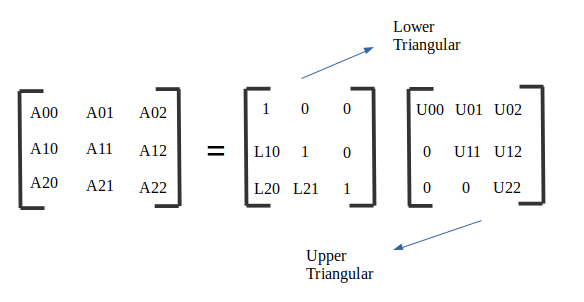
\includegraphics[width=.7\linewidth, keepaspectratio]{figs/matrixluexample.png}
            \caption{Resultado esperado pelo algoritmo LU.}
            \label{lst:matrixluexample}
        \end{figure}
    \end{itemize}
\end{frame}

\begin{frame}\frametitle{LU - Versão Antiga}
    \begin{itemize}
        \item {Permutações de linhas e colunas}
        \item {PLU -> $\mathnormal{P * A = L * U}$
        \item {$\mathnormal{P}$} é o agregado de todas as permutações}
        \item {Envio de blocos da matriz $\mathnormal{A}$ de forma errada}
        \begin{figure}
            \centering
            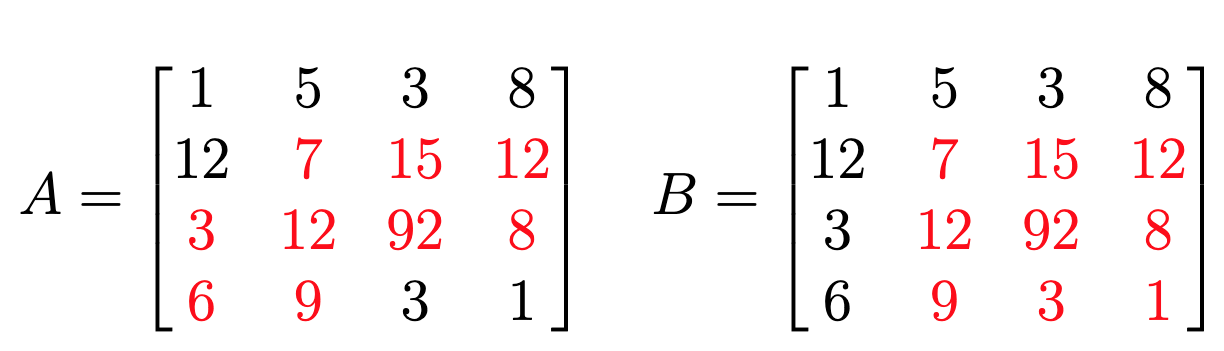
\includegraphics[width=.7\linewidth, keepaspectratio]{figs/luipcwrong.png}
            \caption{Exemplo de um bloco passado a um \textit{slave} em cada versão da LU. (A = Versão antiga, B = Versão nova)}
            \label{fig:rightandwrongblocks}
        \end{figure}
    \end{itemize}
\end{frame}

\begin{frame}\frametitle{LU - Versão Nova}
    \begin{itemize}
        \item {Remoção das permutações de linhas e colunas}
        \item {Correção no envio de blocos aos \textit{slaves}}
        \item {Segmentos sobre o \textit{array} de tarefas e sobre a matriz}
        \item {CCs consultam segmento de tarefas}
        \begin{itemize}
            \item {Verificam se continuam ou finalizam a execução}
            \item {Informação anterior possibilita acessar blocos na matriz}
        \end{itemize}
    \end{itemize}
\end{frame}

\subsection{K-Means}
\begin{frame}\frametitle{K-Means}
    \begin{itemize}
        \item {Algoritmo de clusterização de dados}
        \item {Dados $\mathnormal{n}$ pontos de dimensão $\mathnormal{d}$}
        \begin{itemize}
            \item {Particionar estes pontos em $\mathnormal{k}$ conjuntos}
        \end{itemize}
        \begin{figure}
            \centering
            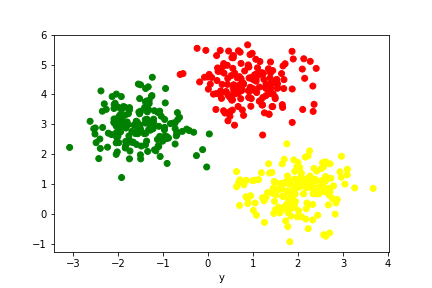
\includegraphics[width=.7\linewidth, keepaspectratio]{figs/kmeans_data.png}
            \caption{Exemplo genérico do resultado final da execução do K-means plotado em um gráfico.}
            \label{fig:kmeansdata}
        \end{figure}
    \end{itemize}
\end{frame}

\begin{frame}\frametitle{Alterações no K-Means}
    \begin{itemize}
        \item {Simplificação no modelo de dados}
        \item {Versão antiga}
        \begin{itemize}
            \item {Pontos eram \textit{structs} -> \texttt{\{dimensão, elementos\}}}
        \end{itemize}
        \item {Versão atual}
        \begin{itemize}
            \item {Pontos salvos em um \textit{array} unidimensional}
            \item {Tamanho do array = nPontos * dimensão}
            \item {Facilidade para criar o segmento sobre os pontos}
        \end{itemize}
    \end{itemize}
\end{frame}

\begin{frame}\frametitle{Alterações no K-Means}
    \begin{itemize}
        \item {Alteração no cálculo dos \textit{centroids}}
        \begin{itemize}
            \item {Média dos elementos de um certo grupo $\mathnormal{k}$}
        \end{itemize}
        \item {Versão antiga}
        \begin{itemize}
            \item {Calculo todo feito nos CCs}
            \item {CCs enviavam as populações parciais ao \textit{master}}
            \item {\textit{Master} respondia a soma desses dados}
        \end{itemize}
        \item {Versão atual}
        \begin{itemize}
            \item {Somente a soma dos vetores parciais é feita nos CCs}
            \item {População total facilmente acessível no \textit{master}}
            \item {Cálculo da média é feita no \textit{cluster} de E/S}
            \item {Redução de 2 operações de escrita e 2 operações de leitura}
        \end{itemize}
    \end{itemize}
\end{frame}

\subsection{Integer-Sort}
\begin{frame}\frametitle{Integer Sort}
    \begin{itemize}
        \item {Algoritmo de ordenação de um grande número de inteiros}
        \item {CAP-Bench -> \textit{bucket-sort}}
        \item {Elementos a serem ordenados são divididos em baldes}
        \begin{itemize}
            \item {Armazena certa quantidade de inteiros}
        \end{itemize}
        \begin{figure}
            \centering
            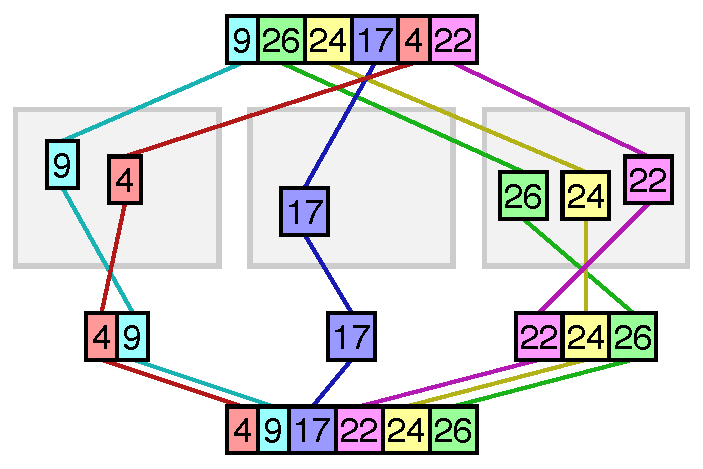
\includegraphics[width=.6\linewidth, keepaspectratio]{figs/bucket-sort.pdf}
            \caption{Exemplo genérico do resultado final da execução do IS na variação \textit{bucket-sort}.}
            \label{fig:bucketsort}
        \end{figure}
    \end{itemize}
\end{frame}

\begin{frame}\frametitle{Alterações no IS}
    \begin{itemize}
        \item {Versão antiga}
        \begin{itemize}
            \item {Ordenação parcial dos \textit{buckets} não otimizada}
            \item {Número de elementos ordenados é sempre o número máximo de elementos em um \textit{bucket} na maior classe de problema (\textit{huge})}
            \item {Valor escolhido pois é divisível por 16 e abrange todas as classes}
            \item {Grande quantidade de elementos \textit{dummy}}
        \end{itemize}
        \item {Versão nova}
        \begin{itemize}
            \item {Ordenação parcial dos \textit{buckets} otimizada}
            \item {Número de elementos ordenados = número de elementos de um \textit{bucket} + no máximo 16 elementos}
            \item {Continua sendo divisível por 16 e abrangendo todas as classes}
            \item {Quantidade insignificante de elementos \textit{dummy}}
        \end{itemize}
    \end{itemize}
\end{frame}

\section{Resultados}
\begin{frame}\frametitle{Métricas definidas}
    \begin{table}[h]
    \centering
    \scalebox{0.75}{
        \begin{tabular}{c c}
            Métrica & Unidade \\\midrule
            Média do tempo de execução dos \textit{slaves} & Segundos \\
            Tempo de execução do processo \textit{master} & Segundos \\
            Tempo total de comunicação entre \textit{master} e \textit{slaves} & Segundos \\
            Quantidade de dados que o \textit{master} envia aos \textit{slaves} & \textit{Megabytes} \\
            Quantidade de dados que o \textit{master} recebe dos \textit{slaves} & \textit{Megabytes} \\
            Potência média durante a execução da aplicação & \textit{Watts} \\
            Consumo de energia durante a execução da aplicação & \textit{joules} \\
            \bottomrule
        \end{tabular}
    }
    \caption{Métricas definidas para comparação das tecnologias.}
    \label{tab:slavetable}
    \end{table}
\end{frame}

\begin{frame}\frametitle{Variações de execução}
    \begin{itemize}
        \item {Classes de tamanho \textit{tiny}, \textit{small}, \textit{standard}, \textit{large} e \textit{huge}}
        \item {Para cada classe, variou-se o número de \textit{clusters} de computação entre 1, 2, 4, 8 e 16}
        \item {5 repetições para cada uma dessas variações}
        \item {16 núcleos de processamento ativos em todas as variações}
    \end{itemize}
\end{frame}

\begin{frame}\frametitle{Significado das tabelas}
    \begin{itemize}
        \item {Exibem redução ou aumento de determinada métrica}
        \begin{itemize}
            \item {$\mathnormal{((Resultado ASYNC / Resultado IPC) - 1) * 100}$}
            \item {Porcentagem de redução/aumento na versão ASYNC}
        \end{itemize}
        \item {Focam no melhor e pior resultado de redução}
    \end{itemize}
\end{frame}

\subsection{Desempenho}
\begin{frame}\frametitle{Tempos de execução de cada CC}
    \begin{itemize}
        \item {Melhoria em todos os \textit{kernels}}
        \item {Redução variou entre 57.14\% e 94.44\%}
    \end{itemize}
    \begin{table}[h]
    \centering
    \scalebox{0.45}{
        \begin{tabular}{l c c c c c c c c c l}
            App & \multicolumn{5}{c}{Redução Mínima} & \multicolumn{5}{c}{Redução Máxima}

            \\\cmidrule(lr){2-6}\cmidrule(lr){7-11}

            & Classe & NClusters & IPC(s) & ASYNC(s) & Redução(\%) & Classe & NClusters & IPC(s) & ASYNC(s) & Redução(\%)\\\midrule

            FAST & Tiny & 8 & 0.72 & 0.05 & 93.06 & Tiny & 16 & 0.36 & 0.02 & 94.44 \\
            FN & Huge & 1 & 34412.07 & 1952.39 & 94.33 & Small & 16 & 267.9 & 15.14 & 94.35 \\
            GF & Tiny & 4 & 1.38 & 0.09 & 93.48 & Tiny & 8 & 0.69 & 0.04 & 94.2 \\ 
            IS & Tiny & 8 & 1.82 & 0.78 & 57.14 & Huge & 1 & 282.06 & 115.03 & 59.22 \\
            KM & Tiny & 16 & 2.86 & 0.19 & 93.36 & Standard & 1 & 1427.49 & 91.55 & 93.59 \\
            LU & Tiny & 2 & 0.28 & 0.09 & 67.86 & Huge & 2 & 40.15 & 9.02 & 77.53 \\

            \bottomrule
        \end{tabular}
    }
    \caption{Reduções ao comparar-se os tempos dos processos \textit{slaves}.}
    \label{tab:slavetable}
    \end{table}
\end{frame}

\begin{frame}\frametitle{Tempos de execução do processo \textit{master}}
    \begin{itemize}
        \item {Melhoria em todos os \textit{kernels}}
        \begin{itemize}
            \item {Exceção: LU}
        \end{itemize}
        \item {Redução variou entre -28.79\% e 70.2\%}
        \item {FAST e GF com tempo 0 em ambas versões}
    \end{itemize}
    \begin{table}[h]
        \centering
        \scalebox{0.45}{
        \begin{tabular}{l c c c c c c c c c l}
            App & \multicolumn{5}{c}{Redução Mínima} & \multicolumn{5}{c}{Redução Máxima}

            \\\cmidrule(lr){2-6}\cmidrule(lr){7-11}

            & Classe & NClusters & IPC(s) & ASYNC(s) & Redução(\%) & Classe & NClusters & IPC(s) & ASYNC(s) & Redução(\%)\\\midrule

            FN & Tiny & 1 & 0.14 & 0.08 & 42.86 & Huge & 1 & 118.54 & 35.32 & 70.2 \\
            IS & Standard & 1 & 12.27 & 10.96 & 10.68 & Huge & 8 & 56.72 & 46.5 & 18.02 \\
            KM & Tiny & 1 & 0.01 & 0.01 & 0.0 & Tiny & 4 & 0.02 & 0.01 & 50.0 \\
            LU & Huge & 2 & 0.66 & 0.85 & -28.79 & Tiny & 2 & 0.02 & 0.02 & 0.0 \\

            \bottomrule
        \end{tabular}
    }
    \caption{Reduções ao comparar-se os tempos do processo \textit{master}.}
    \label{tab:mastertable}
    \end{table}
\end{frame}

\begin{frame}\frametitle{Tempos de comunicação}
    \begin{itemize}
        \item {Melhoria em todos os \textit{kernels}}
        \begin{itemize}
            \item {Exceção: IS}
        \end{itemize}
        \item {Redução variou entre -213.16\% até 99.66\%}
    \end{itemize}
    \begin{table}[h]
    \centering
    \scalebox{0.45}{
        \begin{tabular}{l c c c c c c c c c l}
            App & \multicolumn{5}{c}{Redução Mínima} & \multicolumn{5}{c}{Redução Máxima}

            \\\cmidrule(lr){2-6}\cmidrule(lr){7-11}

            & Classe & NClusters & IPC(s) & ASYNC(s) & Redução(\%) & Classe & NClusters & IPC(s) & ASYNC(s) & Redução(\%)\\\midrule

            FAST & Tiny & 16 & 1.44 & 1.16 & 19.44 & Huge & 8 & 109.55 & 1.25 & 98.86 \\
            FN & Huge & 1 & 34412.4 & 976.35 & 97.16 & Huge & 16 & 2159.8 & 7.34 & 99.66 \\
            GF & Tiny & 16 & 1.31 & 1.1 & 16.03 & Huge & 4 & 1162.81 & 20.57 & 98.23 \\ 
            IS & Tiny & 16 & 1.14 & 3.57 & -213.16 & Huge & 1 & 286.46 & 80.34 & 71.95 \\
            KM & Tiny & 16 & 3.82 & 1.11 & 70.94 & Huge & 16 & 670.86 & 4.28 & 99.36 \\
            LU & Tiny & 16 & 7.22 & 1.36 & 81.16 & Large & 8 & 193.78 & 6.2 & 96.8 \\

            \bottomrule
        \end{tabular}
        }
        \caption{Reduções ao comparar-se os tempos de comunicação.}
        \label{tab:commtable}
    \end{table}
\end{frame}

\subsection{Tráfego de dados}
\begin{frame}\frametitle{Tráfego de dados}
    \begin{itemize}
        \item {Maioria dos resultados foram iguais em ambas versões}
        \begin{itemize}
            \item {Para ambas as métricas de tráfego de dados}
        \end{itemize}
        \item {KM:}
        \begin{itemize}
            \item {Redução entre 6.67\% e 48.51\% para os dados enviados}
            \item {Redução entre -1.56\% e 19.83\% para os dados recebidos}
        \end{itemize}
        \item {LU:}
        \begin{itemize}
            \item {Resultados iguais para todas as classes exceto a \textit{Large}}
            \item {Redução de -100\% nos dados enviados e -171.88\% nos dados recebidos}
        \end{itemize}
        \item {Possivel indicação de \textit{bugs}}
    \end{itemize}
\end{frame}

\subsection{Consumo energético}
\begin{frame}\frametitle{Potência média}
    \begin{itemize}
        \item {Redução variou entre -132.57\% até 3.75\%}
        \item {ASYNC necessita de mais recursos ativos}
    \end{itemize}
    \begin{table}[h]
        \centering
        \scalebox{0.45}{
        \begin{tabular}{l c c c c c c c c c l}
            App & \multicolumn{5}{c}{Redução Mínima} & \multicolumn{5}{c}{Redução Máxima}

            \\\cmidrule(lr){2-6}\cmidrule(lr){7-11}

            & Classe & NClusters & IPC(W) & ASYNC(W) & Redução(\%) & Classe & NClusters & IPC(W) & ASYNC(W) & Redução(\%)\\\midrule

            FAST & Small & 16 & 4.52 & 5.14 & -13.72 & Small & 1 & 4.27 & 4.11 & 3.75 \\
            FN & Large & 16 & 4.79 & 10.25 & -113.99 & Huge & 1 & 4.28 & 4.76 & -11.21 \\
            GF & Huge & 16 & 4.84 & 5.91 & -22.11 & Small & 1 & 4.27 & 4.17 & 2.34 \\
            IS & Large & 16 & 4.48 & 5.99 & -33.71 & Large & 1 & 4.28 & 4.41 & -3.04 \\
            KM & Huge & 16 & 4.82 & 11.21 & -132.57 & Small & 1 & 4.25 & 4.71 & -10.82 \\
            LU & Huge & 16 & 4.42 & 6.05 & -36.88 & Small & 1 & 4.23 & 4.09 & 3.31 \\

            \bottomrule
        \end{tabular}
        }
        \caption{Reduções ao comparar-se a potência média durante execução.}
        \label{tab:avgpower}
    \end{table}
\end{frame}

\begin{frame}\frametitle{Consumo energético}
    \begin{itemize}
        \item {Redução variou entre -30.31\% e 93.64\%}
        \item {Menor tempo de execução justifica maior potência média}
    \end{itemize}
    \begin{table}[h]
        \centering
        \scalebox{0.45}{
            \begin{tabular}{l c c c c c c c c c l}
            App & \multicolumn{5}{c}{Redução Mínima} & \multicolumn{5}{c}{Redução Máxima}

            \\\cmidrule(lr){2-6}\cmidrule(lr){7-11}

            & Classe & NClusters & IPC(J) & ASYNC(J) & Redução(\%) & Classe & NClusters & IPC(J) & ASYNC(J) & Redução(\%)\\\midrule

            FAST & Tiny & 16 & 38.79 & 43.92 & -13.23 & Huge & 1 & 3759.55 & 456.35 & 87.86 \\
            FN & Tiny & 16 & 666.97 & 129.65 & 80.56 & Standard & 1 & 36549.92 & 2325.1 & 93.64 \\
            GF & Tiny & 16 & 38.4 & 44.64 & -16.25 & Huge & 1 & 20504.65 & 1783.83 & 91.3 \\
            IS & Tiny & 16 & 52.2 & 68.02 & -30.31 & Large & 1 & 751.9 & 395.02 & 47.46 \\
            KM & Tiny & 16 & 47.55 & 46.21 & 2.82 & Standard & 1 & 6131.17 & 460.56 & 92.49 \\
            LU & Tiny & 16 & 64.68 & 44.14 & 31.76 & Huge & 8 & 1535.77 & 103.8 & 93.24 \\

            \bottomrule
        \end{tabular}
        }
        \caption{Reduções ao comparar-se o gasto energético total.}
        \label{tab:energy}
    \end{table}
\end{frame}

\section{Conclusão}
\begin{frame}\frametitle{Conclusão}
    \begin{itemize}
        \item {ASYNC se sobressai em comparação a IPC}
        \item {Diretivas assíncronas são uma boa escolha em diversos contextos}
        \item {Comunicações assíncronas tem grande potencial de ganho em desempenho}
        \item {Trabalhos futuros}
        \begin{itemize}
            \item {Comparar MPPA com outros processadores do estado da arte}
        \end{itemize}
    \end{itemize}
\end{frame}

%Fim
\begingroup
    \makeatletter
    \setlength{\hoffset}{-.5\beamer@sidebarwidth}
    \makeatother
    \begin{frame}[plain,t,noframenumbering]
        \titlepage
    \end{frame}
\endgroup

% \section{Extra}
% \begin{frame}\frametitle{Extra}
% \begin{figure}[t]
%   \begin{minipage}[b]{0.9\textwidth}
% 	\centering
%     % \caption{\textit{tiling} 2D.}
%     \includegraphics[height=5cm]{figs/tile.pdf} \\
%     % Fonte:~\cite{rocha17}
% 	\label{fig:block2d}
%   \end{minipage}
% \end{figure}
% \end{frame}

\section{Referências}
\begin{frame}\frametitle{Referências}
    {\tiny
        \bibliographystyle{abbrv}
        \bibliography{bibliography}}
\end{frame}

\end{document}
